\chapter{Results\label{cha:chapter6}}
\section{Data Acquisition}
The data acquisition was performed with 27 subjects in total, 12 (44\%) females and 15 (56\%) males. Participants had an average age of 26.4 years (17, 53, 6.39) and all 27 were right-handed (100\%). 19 (70\%) were students, 8 (30\%) had other occupations.
18 (66\%) subjects stated that their most used input modality is the their thumb while 4 (14\%) preferred using their index finger and 5(18\%) use both thumbs during interactions.\\

\begin{figure}[h!]
  \centering
  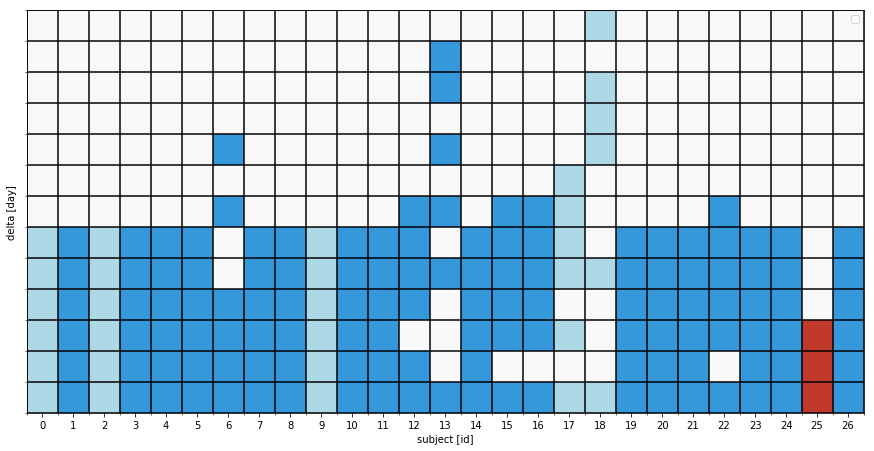
\includegraphics[width=1\textwidth]{participation_push.png}
  \caption{The figure shows on which days the participants took part in the field study. Light blue subjects which did not receive push notifications while subjects with dark blue marks had received push notifications. Red rectangles indicates a dropped out subject.} \label{fig:participation}
\end{figure}

In regards to the participation during the study, 26 subjects managed to finish all laboratory and field study trials while 1 subject dropped out in the field study. Figure \ref{fig:participation} shows on which day individual participants performed trails. 4 participants did not accept push notification and were therefore not reminded on a daily basis.

In total over 46.000 taps were generated in the whole data acquisition phase. To be more precise, approx. 25.000 taps were collected on the 5x4 grid, over 15.000 taps on the 4x3 grid and more than 5.000 taps on the 2x2 grid.

The devices used to obtain the tap information were 12 (45\%) Apple iPhone 6s, 10 (37\%) iPhone 6 and the least common device was the iPhone 7 with 5 (18\%).

In order to visualize the data collected, a t-Distributed Stochastic Neighbor Embedding (t-SNE) embedding is shown in figure \ref{fig:tsne} where the 230-dimensional feature vector has been reduced to 2 dimensions. Furthermore, \ref{ref:taps} shows the interpolated gyroscope and accelerometer signals acquired during a single tap generation trial.

\begin{figure}[h!]
  \centering
  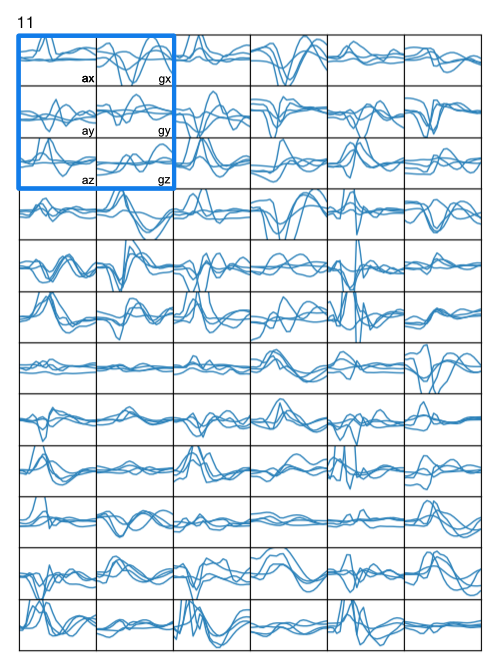
\includegraphics[width=0.8\textwidth]{results/tap4x32.png}
  \caption{The visualization shows the collected gyroscope and accelerometer components for the 4x3 grid. In the top left corner the grid class 11 is shown which corresponds to the top left corner of the mobile device.} \label{fig:taps}
\end{figure}

\afterpage{%
\begin{figure}
  \centering
  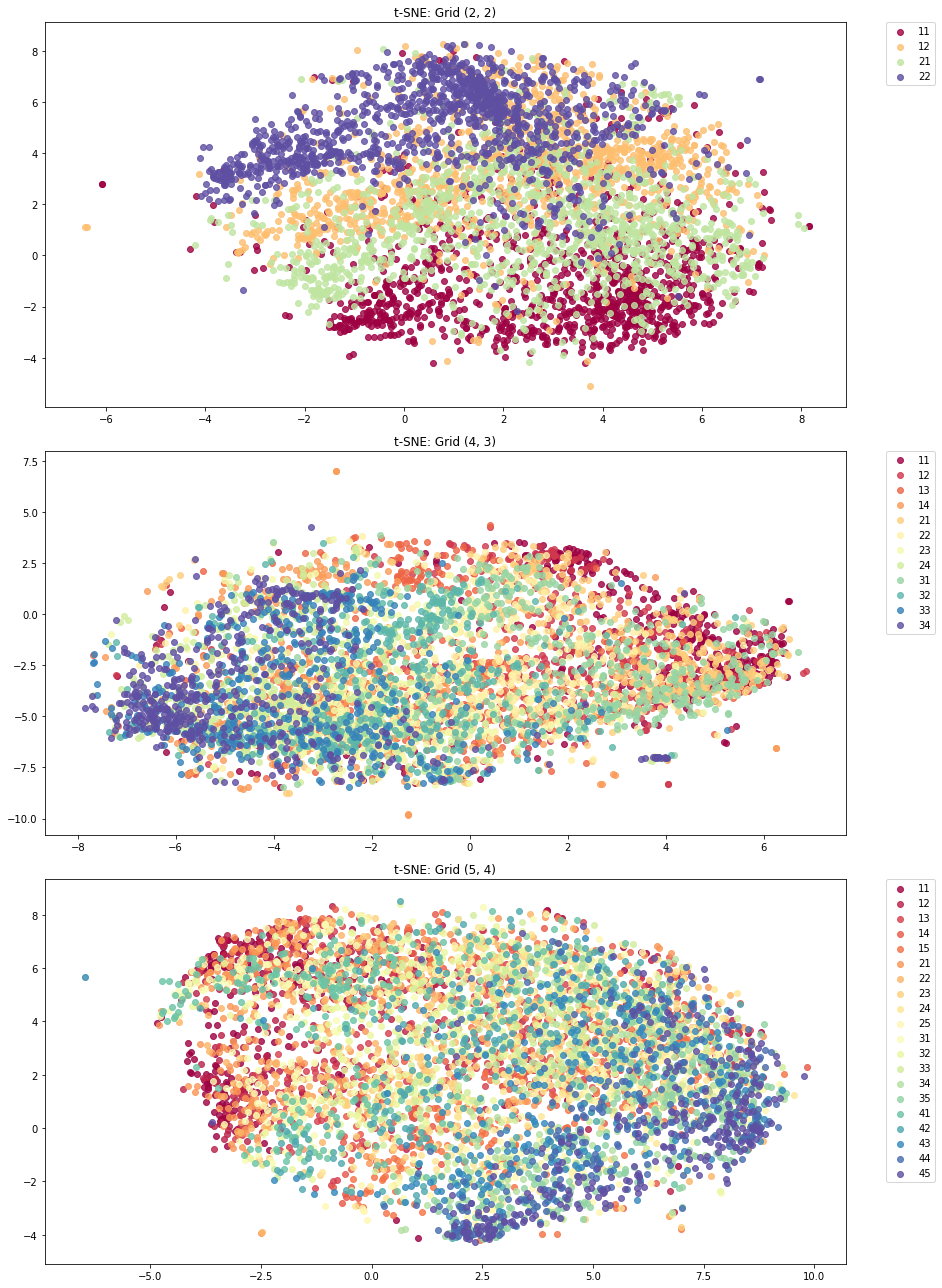
\includegraphics[width=0.9\textwidth]{results/tsne_2.png}
  \caption{ Visualization of 230-dimensional feature vectors reduced to 2 dimensions.
  The used t-SNE dimensionality reduction technique is unsupervised, thus it does
  not consider the labels during the optimization} \label{fig:tsne}
\end{figure}
\clearpage
}

\section{Laboratory and Field Comparison}
For the analysis between the controlled and the uncontrolled environment, a subset of the overall training material has been filtered based on the environment, grid size and the mobile device. After performing a grid search of the hyperparameter space for the SVM and, likewise, for the ANN, a 10-fold cross validation has been performed on the best estimator yielding the highest mean accuracy.

The results show that the neural network classifier outperforms the SVM in all given tasks. This includes all grid sizes, environments and devices alike.

\subsubsection{2x2 Grid}

\begin{figure}[h!]
  \centering
  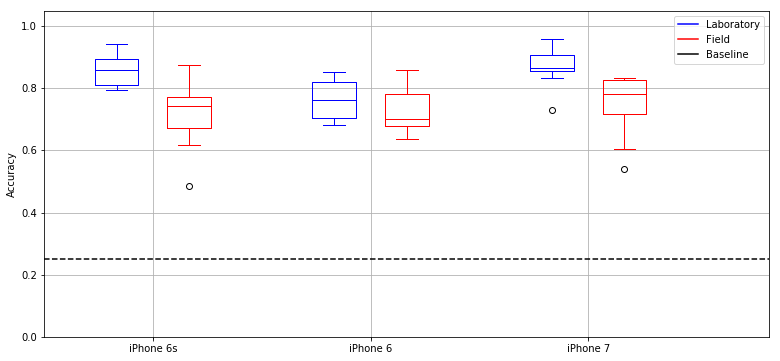
\includegraphics[width=1\textwidth]{results/lab-vs-field-2x2.png}
  \caption{The figure shows the tap inference accuracies for the 2x2 grid of the 10-fold cross-validation.} \label{fig:lab2x2}
\end{figure}

As illustrated in the figure \ref{fig:lab2x2}, for the 2x2 grid the results show that all classification accuracies are above the guessing probability of $\frac{1}{4} = 25\%$ with the iPhone 7 data scoring highest with a mean accuracy of 0.87 (+/- 0.06) in the laboratory environment and 0.75 (+/- 0.10) for the field environment.

\begin{table}[h!]
  \centering
\begin{tabular}{|l|l|c|c|c|c|c|}
  \cline{3-7}
  \multicolumn{2}{c}{} & \multicolumn{4}{|c|}{\textbf{Accuracy}} & \textbf{Kappa} \\
  \hline
  \textbf{Device} & \textbf{Environment} & mean &   min &   max  & std &  mean \\
  \hline
  iPhone 6 & Lab &      0.76 &     0.68 &     0.85 &     0.06 &        0.68 \\
  & Field &      0.73 &     0.64 &     0.86 &     0.07 &        0.64 \\
  \hline
iPhone 7 & Lab &      0.87 &     0.73 &     0.96 &     0.06 &        0.83 \\
  & Field &      0.75 &     0.54 &     0.83 &     0.10 &        0.66 \\
  \hline
iPhone 6s & Lab &      0.86 &     0.80 &     0.94 &     0.05 &        0.81 \\
  & Field &      0.72 &     0.49 &     0.87 &     0.11 &        0.63 \\
  \hline
\end{tabular}
  \caption{Classification results for the 2x2 tapping grid.}
\end{table}

Results show that the model trained with data from the iPhone 7 outperform the models trained with the iPhone 6 and iPhone 6s, respectively. The iPhone 6 models shows least accuracy scores of 0.76 (+/- 0.06) for the controlled and 0.73 (+/- 0.07) for the uncontrolled environment.

% For the comparison of devices, the results yield that the iPhone 7 scores higher accuracies compared to the iPhone 6 and and the iPhone 6s for both environments. The iPhone 6 scores lowest with a mean accuracy of 0.76 (+/- 0.85) while the iPhone 7 performs best with a mean accuracy of 0.87 (+/- 0.96) in the controlled environment. For the field environnement the iPhone 7 scores a mean accuracy of 0.75 (+/- 0.83) while the iPhone 6 shows 0.73 (+/- 0.86).

Moreover, the results reveal that all mean accuracy scores across all devices are lower in the field compared to the laboratory environment. The fact that the classification results for both environments differ significantly is confirmed by a Wilcoxon signed-rank test yielding that the fold accuracies in the laboratory were significantly higher than the fold accuracies in the field environment $Z = 24, p < 0.05$.

\subsubsection{4x3 Grid}

The classification results for the 4x3 grid size show that all inference accuracies are above the probability baseline of guessing ($\frac{1}{12}= 8.33\%$ for the 12 distinguishable buttons). Here, the iPhone 7 scores best with a mean accuracy of 0.62 (+/- 0.10) in the laboratory environment and 0.48 (+/- 0.10) in the field environment.

\begin{figure}[h!]
  \centering
  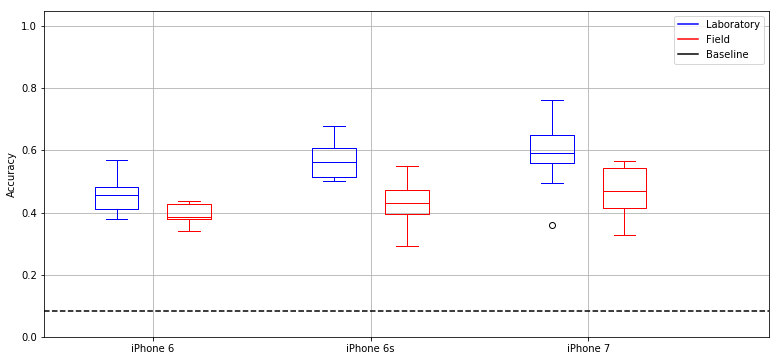
\includegraphics[width=1\textwidth]{results/lab-vs-field-4x3.png}
  \caption{The figure shows the tap inference accuracies for the 4x3 grid of the 10-fold cross-validation.} \label{fig:participation}
\end{figure}

Aligning with the results of the small grid, the results show that the models trained for the iPhone 7 perform best, followed by the models trained on the iPhone 6s and iPhone 6, consecutively. The iPhone 6 performs worst in comparison to the other devices yielding accuracies of 0.47 (+/- 0.06) in the controlled and 0.41 (+/- 0.04) in the uncontrolled environment.

\begin{table}[h!]
  \centering
\begin{tabular}{|l|l|c|c|c|c|c|}
  \cline{3-7}
  \multicolumn{2}{c}{} & \multicolumn{4}{|c|}{\textbf{Accuracy}} & \textbf{Kappa} \\
  \hline
  \textbf{Device} & \textbf{Environment} & mean &   min &   max  & std &  mean \\
  \hline
  iPhone 6 & Lab &      0.47 &     0.36 &     0.56 &     0.06 &        0.42 \\
  & Field &      0.41 &     0.35 &     0.48 &     0.04 &        0.35 \\
  \hline
iPhone 7 & Lab &      0.62 &     0.41 &     0.78 &     0.10 &        0.59 \\
  & Field &      0.48 &     0.31 &     0.63 &     0.10 &        0.43 \\
  \hline
iPhone 6s & Lab &      0.56 &     0.47 &     0.65 &     0.06 &        0.52 \\
  & Field &      0.42 &     0.29 &     0.54 &     0.07 &        0.36 \\
  \hline
\end{tabular}
  \caption{Classification results for the 4x3 tapping grid.}
\end{table}

The Wilcoxon signed-rank test shows that the classification results for both environments differ significantly. The fold accuracies in the laboratory were statistically higher than the fold accuracies in the field environment $Z = 21, p < 0.05$.

\subsubsection{5x4 Grid}
For the grid with 20 distinguishable buttons the inference accuracies range from 0.46 (+/- 0.11) on the iPhone 7 to 0.28 (+- 0.03) for the iPhone 6. Results show that all inference accuracies are above the baseline of $\frac{1}{20} = 5\%$ for this classification problem.

\begin{table}[h!]
  \centering
\begin{tabular}{|l|l|c|c|c|c|c|}
  \cline{3-7}
  \multicolumn{2}{c}{} & \multicolumn{4}{|c|}{\textbf{Accuracy}} & \textbf{Kappa} \\
  \hline
  \textbf{Device} & \textbf{Environment} & mean &   min &   max  & std &  mean \\
  \hline
  iPhone 6 & Lab &      0.35 &     0.28 &     0.45 &     0.06 &        0.32 \\
  & Field &      0.28 &     0.23 &     0.33 &     0.03 &        0.24 \\
  \hline
iPhone 7 & Lab &      0.46 &     0.21 &     0.63 &     0.11 &        0.43 \\
  & Field &      0.34 &     0.25 &     0.47 &     0.08 &        0.31 \\
  \hline
iPhone 6s & Lab &      0.42 &     0.34 &     0.50 &     0.05 &        0.39 \\
  & Field &      0.30 &     0.18 &     0.38 &     0.06 &        0.26 \\
  \hline
\end{tabular}
  \caption{Classification results for the 5x4 tapping grid.}
\end{table}

Aligning with the results from the two previous grids, the iPhone 7 models show higher mean accuracies compared to the other devices. 

Furthermore, The Wilcoxon signed-rank test shows that the classification results for both environments alter significantly. The fold accuracies in the laboratory were significantly higher than the fold accuracies in the field environment $Z = 22, p < 0.05$.

\begin{figure}[h!]
  \centering
  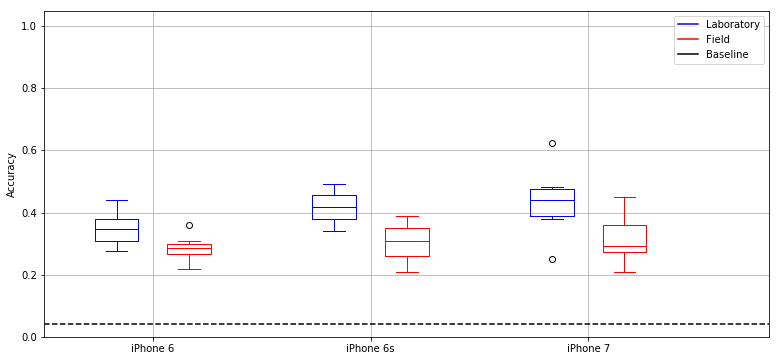
\includegraphics[width=1\textwidth]{results/lab-vs-field-5x4.png}
  \caption{The figure shows the tap inference accuracies for the 4x3 grid of the 10-fold cross-validation.} \label{fig:participation}
\end{figure}

\section{Input Modalities Comparison}
As for the comparison between controlled and uncontrolled environments, the same classification experiment was performed to detect differences in the predictive models between the two input modalities: Index finger and thumb. As subjects were free to decide which input modality to use during the field study, the sample size has been adjusted in order to train each classifier with the same amount of training material.

Classifier trained for the individual grid sizes show similar results. For this reason, only the results for the 5x4 grid will be shown here. The results for the other grid sizes are listed in the Appendix. %TODO

For the 5x4 grid, the results show that across all devices the mean inference accuracies for estimators trained with the thumb taps were lower compared to the classifiers trained with data containing index finger taps. For the iPhone 7, the estimator yields a mean accuracy of 0.54 (+/- 0.04) for index finger samples compared to 0.38 (+/- 0.04)  for data representing the thumb as input modality.  Same results apply for the other tested devices. A Wilcoxon signed-rank test shows that the classification results for both input modalities differ significantly. The fold accuracies on thumb data were statistically lower than the fold accuracies on index finger data Z = 29, p < 0.05.


\begin{figure}[h!]
  \centering
  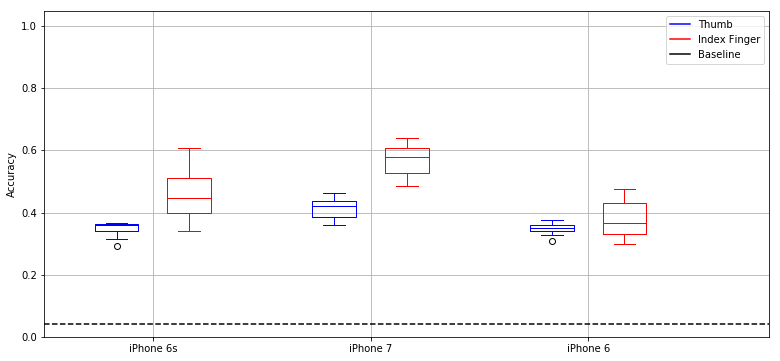
\includegraphics[width=1\textwidth]{results/index-vs-thumb-5x4.png}
  \caption{The figure shows the tap inference accuracies for the 5x4 grid of the 10-fold cross-validation.} \label{fig:participation}
\end{figure}

\begin{table}[h!]
  \centering
\begin{tabular}{|l|l|c|c|c|c|c|}
  \cline{3-6}
  \multicolumn{2}{c}{} & \multicolumn{4}{|c|}{\textbf{Accuracy}}  \\
  \hline
  \textbf{Device} & \textbf{Input Modality} & mean &   min &   max  & std &  \textbf{Classifier} \\
  \hline
  iPhone 6 & Index &      0.38 &     0.28 &     0.47 &     0.06 &  ANN \\
  & Thumb &      0.35 &     0.33 &     0.37 &     0.01 &  ANN \\
  \hline
iPhone 6s & Index &      0.44 &     0.35 &     0.54 &     0.06 &  SVM \\
  & Thumb &      0.37 &     0.33 &     0.41 &     0.02 &  ANN \\
  \hline
  iPhone 7 & Index &      0.54 &     0.45 &     0.59 &     0.04 &  SVM \\
  & Thumb &      0.38 &     0.30 &     0.42 &     0.04 &  ANN \\
  \hline
\end{tabular}
  \caption{Classification results for the 5x4 tapping grid for both input modalities: thumb and index finger.}
\end{table}

\section{Body Posture Comparison}
For the comparison between the two body postures (sitting and standing) the overall training material was filtered based on the device and body posture the user had while tapping. As for the comparison of input modalities, the amount of training material was balanced for both postures. Aligning with the previous results, the ANN outperforms the SVM in all tasks.

The results show similar results for the three grids sizes. Therefore only the results for 5x4 grid are presented in this section. The findings show that the mean accuracies between the two body modalities did not show clear distinctions. In some cases data referencing a sitting posture resulted in higher accuracies while in other cases the standing data yielded higher results (See figure \ref{fig:bodypos5x4}). This is also indicated in a Wilcoxon signed-rank test showing that the classification results for both factors did not alter significantly $Z = 176, p > 0.05$. This lack in statistical significance is also to be found for the other grid sizes (Results are to be found in the Appendix).

\begin{figure}[h!]
  \centering
  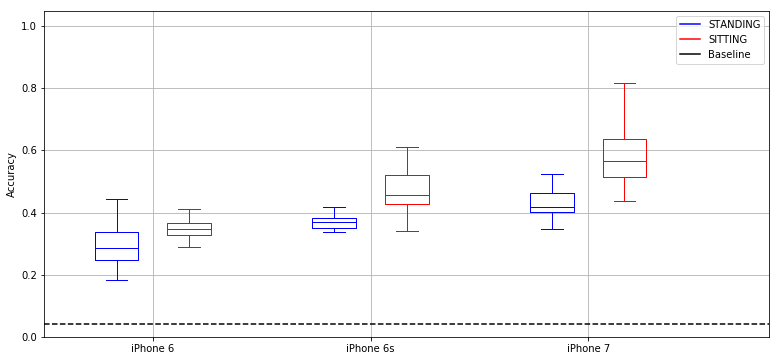
\includegraphics[width=1\textwidth]{results/standing-vs-sitting-5x4.png}
  \caption{The figure shows the tap inference accuracies for the 5x4 grid of the 10-fold cross-validation.} \label{fig:bodypos5x4}
\end{figure}

\begin{table}[h!]
  \centering
\begin{tabular}{|l|l|c|c|c|c|c|}
  \cline{3-7}
  \multicolumn{2}{c}{} & \multicolumn{4}{|c|}{\textbf{Accuracy}} & \textbf{Kappa} \\
  \hline
  \textbf{Device} & \textbf{Input Modality} & mean &   min &   max  & std &  mean \\
  \hline
  iPhone 6 & Standing &      0.32 &     0.25 &     0.38 &     0.04 &        0.29 \\
  & Sitting &      0.34 &     0.32 &     0.38 &     0.02 &        0.31 \\
  \hline
iPhone 7 & Standing &      0.45 &     0.19 &     0.59 &     0.11 &        0.43 \\
  & Sitting &      0.37 &     0.34 &     0.40 &     0.02 &        0.34 \\
  \hline
iPhone 6s & Standing &      0.39 &     0.28 &     0.49 &     0.06 &        0.36 \\
  & Sitting &      0.37 &     0.32 &     0.41 &     0.03 &        0.34 \\
  \hline
\end{tabular}
  \caption{Classification results for the 5x4 tapping grid for both input modalities: thumb and index finger.}
\end{table}


\section{Discussion}
For the hypothesis tests, the assumptions made in section \ref{sec:sec:hypothesis} will be either rejected or approved based on the results stated in the previous chapter.

\begin{center}
  \begin{framed}
    \textbf{H.1}  The environment of recorded sensory data has an effect on the prediction accuracy.\\
    \textbf{H1.1:} The prediction accuracy for a classifier trained with the data in the laboratory environment will score higher than one trained with data collected in the field.
  \end{framed}
\end{center}

Both assumptions can be approved as the results yield a significant difference between the performance measures of the estimators for both environments. Across all available grid sizes analysis has shown that a tap inference is reasonably possible in the field as well as in the laboratory environment. 

For the 4x3 grid, a mean accuracy of xx was shown for the laboratory and xx for the field data, respectively. In contrast, for the 5x4 grid an average accuracy of xx was shown for the field was well as xx for the controlled dataset. It can be assumed that these accuracies could be sufficient to obtain PINs in a malicious attack or at least significantly reduce the search space of cracking a PIN. However, these inference accuracies measured should not be interpreted as an upper bound to what is feasible, but should indicate that tap location inference in the field is considerably more difficult. This is especially the case for the more complex classification problems as for the higher grid sizes in this experiment.

% The performance measured is not an upper bound to what is feasible, however, the results indicate a clear performance drop in the accuracy measures found for data from the field. This is especially the case for the more complex classification problems as for the higher grid sizes in this experiment.

% The drop in performance can be explained by looking at the usual behavior of smartphone users when interacting with their devices.

Since device motion sensors are capable of capturing the slightest device vibrations, a vibrant environment or activity, one to which subjects where exposed during the field experiment, is presumably prone to polluting the sensor signals with increased noise. The results hint that the increase in noise undermines the actual signal caused by the tap event aggravating clear predictions of the tap location. Consequently, as subjects where free to perform tap generation trails where and how they wanted, this freedom is reflected in the recorded data sets with increased variability negatively impacting the classification accuracies.

These findings have implications regarding the actual security threat posed by motion sensor emanations. Similar experiments, such as \cite{Tapprints, Accessory}, proclaimed that PINs and Passwords could be obtained by capturing gyroscope and accelerometer signals. However, as the data obtained for training the classifiers in these experiments originated from a controlled environment, the proclaimed security threat has to be reassessed with the results found in this experiment. If an inference system was to be deployed for a real world attack, the system would have to overcome increased environmental noise and users switching input modalities and body postures, as modelled in this experiment. \\

\begin{center}
  \begin{framed}
    \textbf{H2:} The input modality has an effect on the prediction accuracy.\\
    \textbf{H2.2:} The prediction accuracy for a classifier trained with index finger tap data will score higher than one trained with thumb tap data.
  \end{framed}
\end{center}

The analysis has shown that classification results, when comparing the input modalities, differed significantly. As the index finger taps could be predicted at higher measures compared to the thumb taps, both hypothesis can be approved.

This outcome can be explained by comparing the motion of the individual input modalities. When a user taps the device with the index finger, the striking force of the finger is applied in a linear fashion causing a shift towards the z-axis. In addition, the other hand is used as a support, which partially resists the applied force and stops the device from tilting. In comparison, when a user taps with the thumb, the striking force causes the device to rotate in addition to the shift movement as the device is held in the same hand. This rotation causes a higher variance in the recorded data which result in an inferior predictability.

% We can derive from this, that the predictability of a tap is strongly influences by the striking force of the physical tap and resisting force of the supporting hand.

% - 

\begin{center}
  \begin{framed}
    \textbf{H3}: The body posture has an effect on the prediction accuracy.\\
    \textbf{H3.1:} The prediction accuracy for a classifier trained with taps where a user sat will score higher than one trained with taps where a user stood.
  \end{framed}
\end{center}

The analysis has shown that the difference in classification measures for both body postures, sitting and standing, differ significantly. The classification for sitting data yielded higher accuracies as compared to the standing data sets. Due to this finding, both assumptions can be approved. 

These findings indicate that the body posture poses an important influence factor on the variability in the motion data collected. This result can be explained based on two assumptions. Firstly, it is likely that subjects used their device while walking during the field study which poses a source for increased noise. Secondly, during the data acquisition in the laboratory environment, it is known that subject did not walk while tapping the device. As this data was also contained in the training examples, the assumption can be made that standing on the spot also causes movement in the body of the user.

%-----
Speaking of algorithms, the results show that the SVM with RBF kernel was capable of scoring higher accuracies for most tasks at hand. The t-SNE embedding, see figure \ref{fig:tsne}, and the fact that high gamma and C values where chosen during the grid search hint that the classification problem posed is indeed non-trivial. This results in the classifiers having to learn complex non-linear decision boundaries which both classifiers are capable of. Yet, as the ANN has the tendency to overfit the training data when limited data is available, this result can be explained.

Moreover, the observation has been made that data collected iPhone 7 achieves higher performance compared to the other device tested, especially for the iPhone 6 data. This can be explained by the fact on high CPU loads the sampling rate of the sensors drop. It could be observed that for the iPhone 6 the sample frequency has dropped under 80Hz which effects the classification performance.
% Furthermore, the results have shown that the ANN classifier outperformed the SVM with RBF Kernel in all given tasks. 

In summary, in this work we have seen that the tap inference is feasible in the field environment. By measuring and comparing the performance of classifiers trained on different sets of data, several source of variability have been identified. Following the hypothesis stated, this implies that a real world implementation would have to overcome increased variability originating from the input modality, the body posture, the environment in which the tap was recorded and the device model (including CPU, screen size and sensors). 

% Sources of Variability: A real-world implementation of this attack
% would have to address several sources of variability such as
% different hand sizes, typing styles, screen sizes, and keyboard user
% interfaces. Nevertheless, we do not claim that our models are generalizable
% to address these issues. Individual calibration will likely
% always be a necessity, but we believe our model can be extended to
% address these and other sources of variability given the appropriate
% training data.
% In general, though there certainly exists subtle variabilities, most
% people enter text on smartphones in a similar fashion. We observe
% several categories of typing styles. For example, some people prefer
% to hold a phone with one hand while using the index finger of the
% other hand to enter text, while others prefer to hold a phone with both
% hands and enter text using their thumbs. Typing style also depends
% on whether the phone is held in a portrait or landscape orientation. A
% sample of the acceleration measurements can be used to identify the
% holding style of the user. This enables the adversary to switch to the
% appropriate translation model.
% Some variables can be identified directly by the running application
% (e.g., the screen size and keyboard UI). In the case of variability
% that is not easily identified from the acceleration measurements or by
% the application, the adversary can train the model separately for each
% configuration and use the results of the model that produces the most
% sensible output. We make simplifying assumptions because the goal
% of our work is to show that such attacks are feasible due to the nature
% of information leaked by accelerometers.
% Real-World Threat: Major websites typically limit the number
% of retries for entering a password. Our results indicate that a small
% fraction of passwords can be cracked in a limited number of trials
% (e.g., 1 of 99 passwords was cracked in 1 attempt and 6 of 99 in 4.5
% median attempts). Attackers can perform this attack in a scalable
% manner where cracking just 1% of passwords can be lucrative.
% Our model makes no assumptions about the text being entered–
% it simply maps sensor data to screen locations to keys. This attack
% can be used to extract other types of text, such as text messages and
% e-mail, where a perfect translation is not necessary to produce an
% approximate text representation and enable the extraction of sensitive
% information. Furthermore, the structured form of natural-language
% text makes it vulnerable to further analysis (e.g., analysis that uses
% a dictionary-backed sequencing model, such as the n-gram language
% model, to further disambiguate the entered text.
% There do exist simpler methods for attackers to obtain sensitive
% information from smartphones. We discuss some of these threats in
% §1 and §6. However, the accelerometer is a particularly interesting
% case since it presents a physical side channel that cannot be easily
% shielded or detected. It is prudent to consider an adversary with more
% resources that is willing to invest the extra time needed to develop a
% robust eavesdropping application with these stealthy properties. Our
% model represents a proof-of-concept design to demonstrate that this
% is a real threat.

